%  CONFIGURE NEWcitep SINGLE-PAGE FORMAT

\onecolumn % go back to one column
%\fancyhead{} % make sure we get no headers
\renewcommand{\floatpagefraction}{0.1}
%\lfoot[\bSupInf]{\dAuthor}
%\rfoot[\dAuthor]{\cSupInf}
\newpage

%\captionsetup*{format=largeformat} % make figure legend slightly larger than in the paper
\setcounter{figure}{0} % reset figure counter for Supp. Figures
\setcounter{equation}{0} % reset equation counter for Supp. Equations
%\setcounter{page}{1} % reset page count
%\makeatletter
%\renewcommand{\thefigure}{S\@arabic\c@figure} % make Figure legend start with Figure S
%\makeatother
%\def\theequation{S\arabic{equation}}
\renewcommand{\figurename}{Supplementary Figure}

%  MAIN TEXT

\newpage
\section*{Supplementary Information}

%%%%%%%%%%%%%%%%%%%%%%%%%%%%%%%%%%%%%%%%%%%%%%%%%%%%%%%%%%%%%%%%%%%%%%%%%%%%%%%%%
%%
%% Supp fig 1: Scatter plots of winner regions
%%
%%%%%%%%%%%%%%%%%%%%%%%%%%%%%%%%%%%%%%%%%%%%%%%%%%%%%%%%%%%%%%%%%%%%%%%%%%%%%%%%%
%
%\begin{figure}[!tbp]
%
%\begin{subfigure}[]{.24\textwidth}
%\textbf{a}
%\\
%\includegraphics[width=\textwidth]{\floatRelativePath/pltsctr_x_per_rsid_y_gwas.py/count_per_rsid_chr5_start132239645_end132497907_categories9.png}
%\end{subfigure}
%%
%\begin{subfigure}[]{.24\textwidth}
%\textbf{b}
%\\
%\includegraphics[width=\textwidth]{\floatRelativePath/pltsctr_x_per_rsid_y_gwas.py/count_per_rsid_chr9_start21950524_end22207038_categories7.png}
%\end{subfigure}
%%
%\begin{subfigure}[]{.24\textwidth}
%\textbf{c}
%\\
%\includegraphics[width=\textwidth]{\floatRelativePath/pltsctr_x_per_rsid_y_gwas.py/count_per_rsid_chr11_start65747403_end65909045_categories7.png}
%\end{subfigure}
%%
%\begin{subfigure}[]{.24\textwidth}
%\textbf{d}
%\\
%\includegraphics[width=\textwidth]{\floatRelativePath/pltsctr_x_per_rsid_y_gwas.py/count_per_rsid_chr20_start63588387_end63857282_categories8.png}
%\end{subfigure}
%
%\begin{subfigure}[]{.24\textwidth}
%\textbf{e}
%\\
%\includegraphics[width=\textwidth]{\floatRelativePath/pltsctr_x_per_rsid_y_egene.py/count_per_rsid_chr5_start132239645_end132497907_categories9.png}
%\end{subfigure}
%%
%\begin{subfigure}[]{.24\textwidth}
%\textbf{f}
%\\
%\includegraphics[width=\textwidth]{\floatRelativePath/pltsctr_x_per_rsid_y_egene.py/count_per_rsid_chr9_start21950524_end22207038_categories7.png}
%\end{subfigure}
%%
%\begin{subfigure}[]{.24\textwidth}
%\textbf{g}
%\\
%\includegraphics[width=\textwidth]{\floatRelativePath/pltsctr_x_per_rsid_y_egene.py/count_per_rsid_chr11_start65747403_end65909045_categories7.png}
%\end{subfigure}
%%
%\begin{subfigure}[]{.24\textwidth}
%\textbf{h}
%\\
%\includegraphics[width=\textwidth]{\floatRelativePath/pltsctr_x_per_rsid_y_egene.py/count_per_rsid_chr20_start63588387_end63857282_categories8.png}
%\end{subfigure}
%
%\begin{subfigure}[]{.24\textwidth}
%\textbf{i}
%\\
%\includegraphics[width=\textwidth]{\floatRelativePath/pltsctr_x_per_rsid_y_etissue.py/count_per_rsid_chr5_start132239645_end132497907_categories9.png}
%\end{subfigure}
%%
%\begin{subfigure}[]{.24\textwidth}
%\textbf{j}
%\\
%\includegraphics[width=\textwidth]{\floatRelativePath/pltsctr_x_per_rsid_y_etissue.py/count_per_rsid_chr9_start21950524_end22207038_categories7.png}
%\end{subfigure}
%%
%\begin{subfigure}[]{.24\textwidth}
%\textbf{k}
%\\
%\includegraphics[width=\textwidth]{\floatRelativePath/pltsctr_x_per_rsid_y_etissue.py/count_per_rsid_chr11_start65747403_end65909045_categories7.png}
%\end{subfigure}
%%
%\begin{subfigure}[]{.24\textwidth}
%\textbf{l}
%\\
%\includegraphics[width=\textwidth]{\floatRelativePath/pltsctr_x_per_rsid_y_etissue.py/count_per_rsid_chr20_start63588387_end63857282_categories8.png}
%\end{subfigure}
%
%\caption{Count of GWAS classes (\textbf{a-d}), eQTL genes (\textbf{d-h}) and eQTL tissues (\textbf{i-l}) in four
%pleiotropic genomic regions: \textbf{a,e,i}: 5:132,239,645-132,497,907 (5q31.1), \textbf{b,f,j}: 9:21,950,524-22,207,038 (9q21.3),
%    \textbf{c,g,k}: 11:65,747,403-65,909,045 (11q13.1), and \textbf{d,h,l}: 20:63,588,387-63,857,282 (20q13.33).
%    Genomic coordinates are given for the hg38 assembly.}
%\label{fig:region_gwas_egenes_tissues}
%%
%\end{figure}


%%%%%%%%%%%%%%%%%%%%%%%%%%%%%%%%%%%%%%%%%%%%%%%%%%%%%%%%%%%%%%%%%%%%%%%%%%%%%%%%%
%%
%% Supp fig 2: beta and pval
%%
%%%%%%%%%%%%%%%%%%%%%%%%%%%%%%%%%%%%%%%%%%%%%%%%%%%%%%%%%%%%%%%%%%%%%%%%%%%%%%%%%
%
%\begin{figure}[!tbp]
%
%    \begin{subfigure}[]{.32\textwidth}
%        \textbf{a}
%        \\
%        \includegraphics[width=\textwidth]{\floatRelativePathTwentyFive/plthst_perc_tophits_eqtl.py/hist_perc_tophits_eqtl_excl_mhc.png}
%    \end{subfigure}
%%
%    \begin{subfigure}[]{.32\textwidth}
%        \textbf{b}
%        \\
%        \includegraphics[width=\textwidth]{\floatRelativePath/plthst_perc_tophits_eqtl.py/hist_perc_tophits_eqtl_excl_mhc.png}
%    \end{subfigure}
%%
%    \begin{subfigure}[]{.32\textwidth}
%        \textbf{c}
%        \\
%        \includegraphics[width=\textwidth]{\floatRelativePathSeventyFive/plthst_perc_tophits_eqtl.py/hist_perc_tophits_eqtl_excl_mhc.png}
%    \end{subfigure}
%
%    \caption{}
%
%\end{figure}

%%%%%%%%%%%%%%%%%%%%%%%%%%%%%%%%%%%%%%%%%%%%%%%%%%%%%%%%%%%%%%%%%%%%%%%%%%%%%%%%
%
% Fig 2: ucsc screenshots
%
%%%%%%%%%%%%%%%%%%%%%%%%%%%%%%%%%%%%%%%%%%%%%%%%%%%%%%%%%%%%%%%%%%%%%%%%%%%%%%%%

\begin{figure}[!ht]
    \centering

    \begin{subfigure}[]{0.99\textwidth}
        \textbf{a}
        \\
        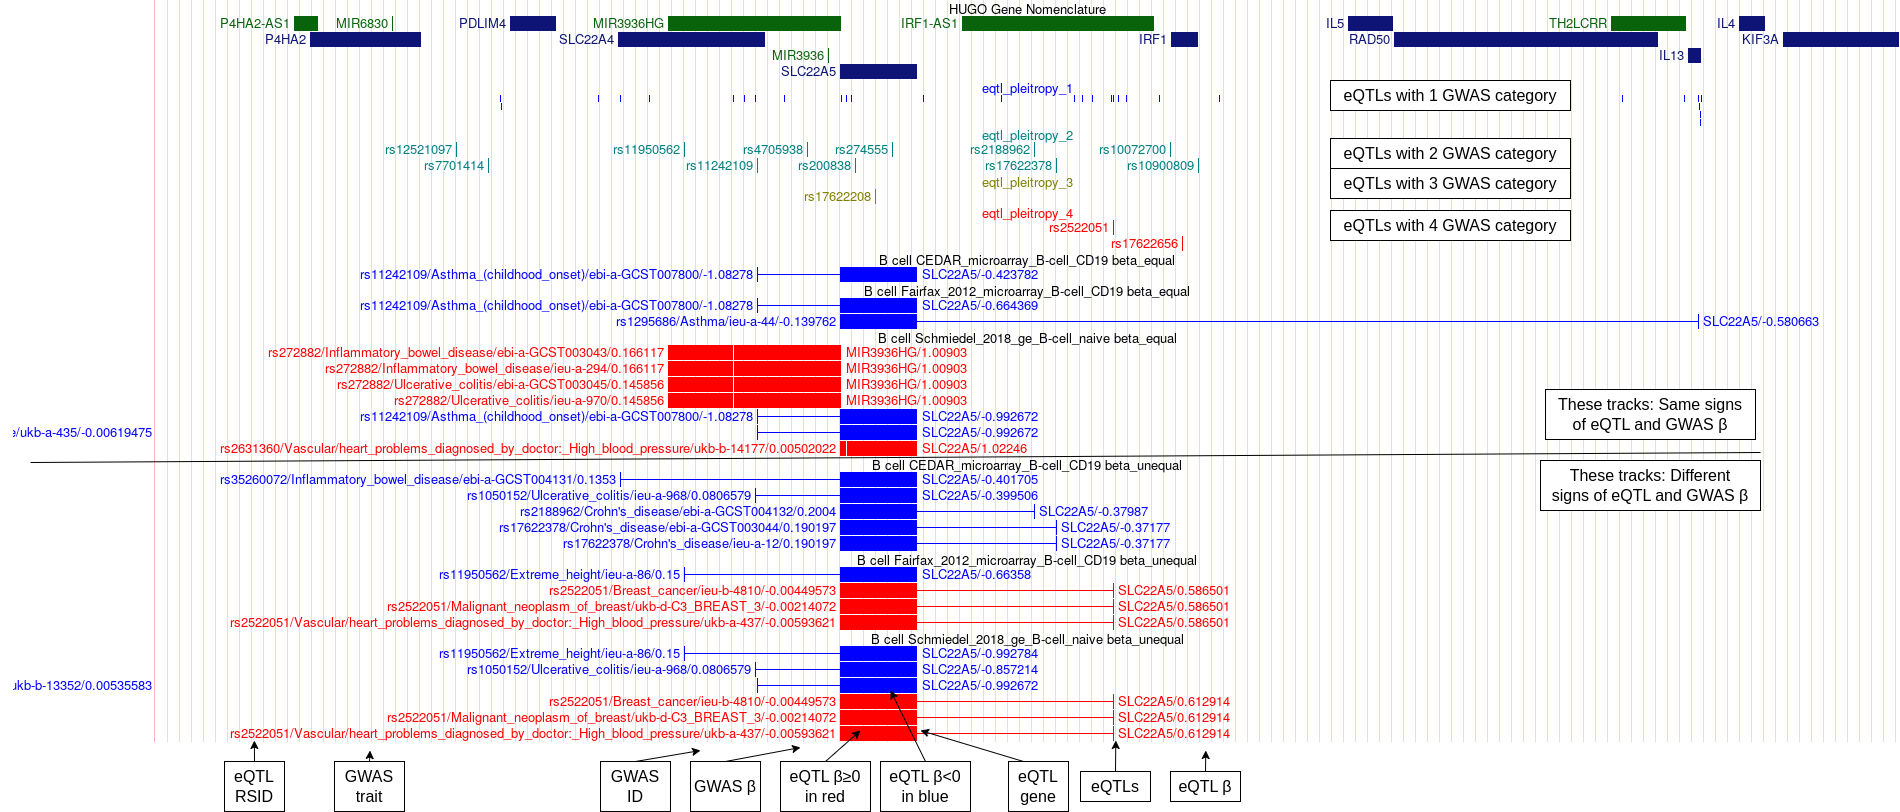
\includegraphics[width=\textwidth]{fig/ucsc_gwas2eqtl_il4_bcell_help.png}
    \end{subfigure}

    \begin{subfigure}[]{0.99\textwidth}
        \textbf{b}
        \\
        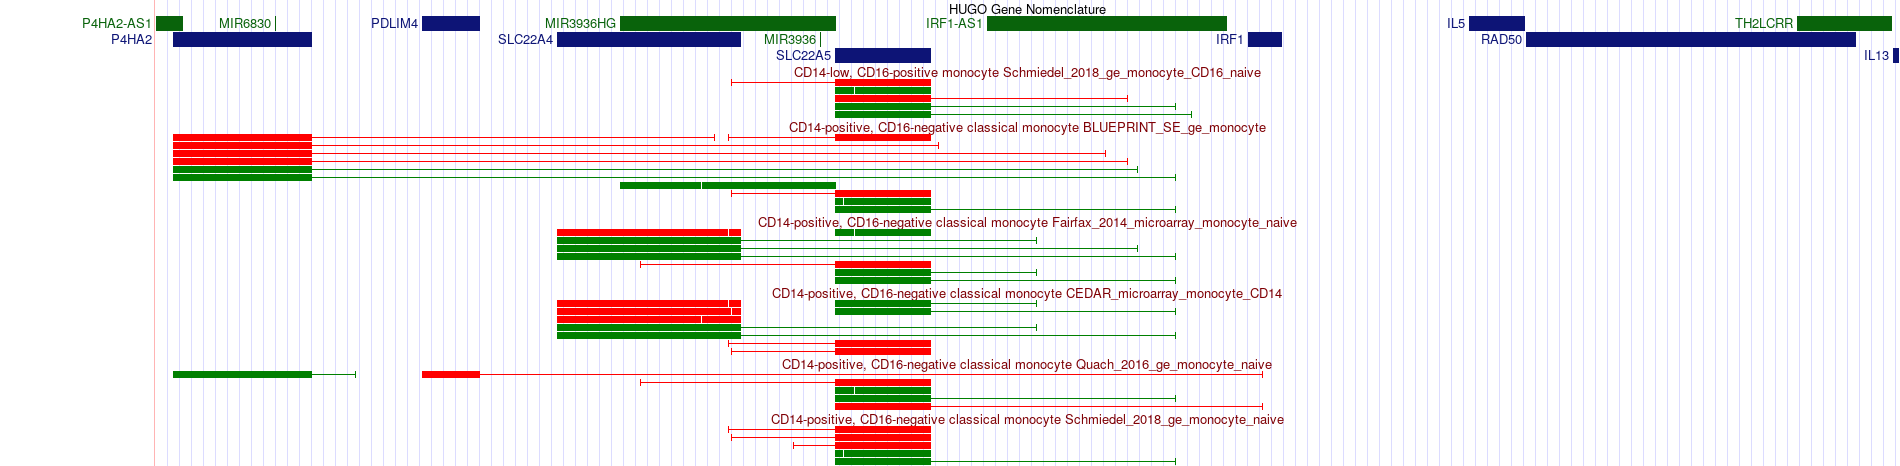
\includegraphics[width=\textwidth]{fig/ucsc_gwas2eqtl_il4_monocyte.png}
    \end{subfigure}

    \begin{subfigure}[]{0.99\textwidth}
        \textbf{c}
        \\
        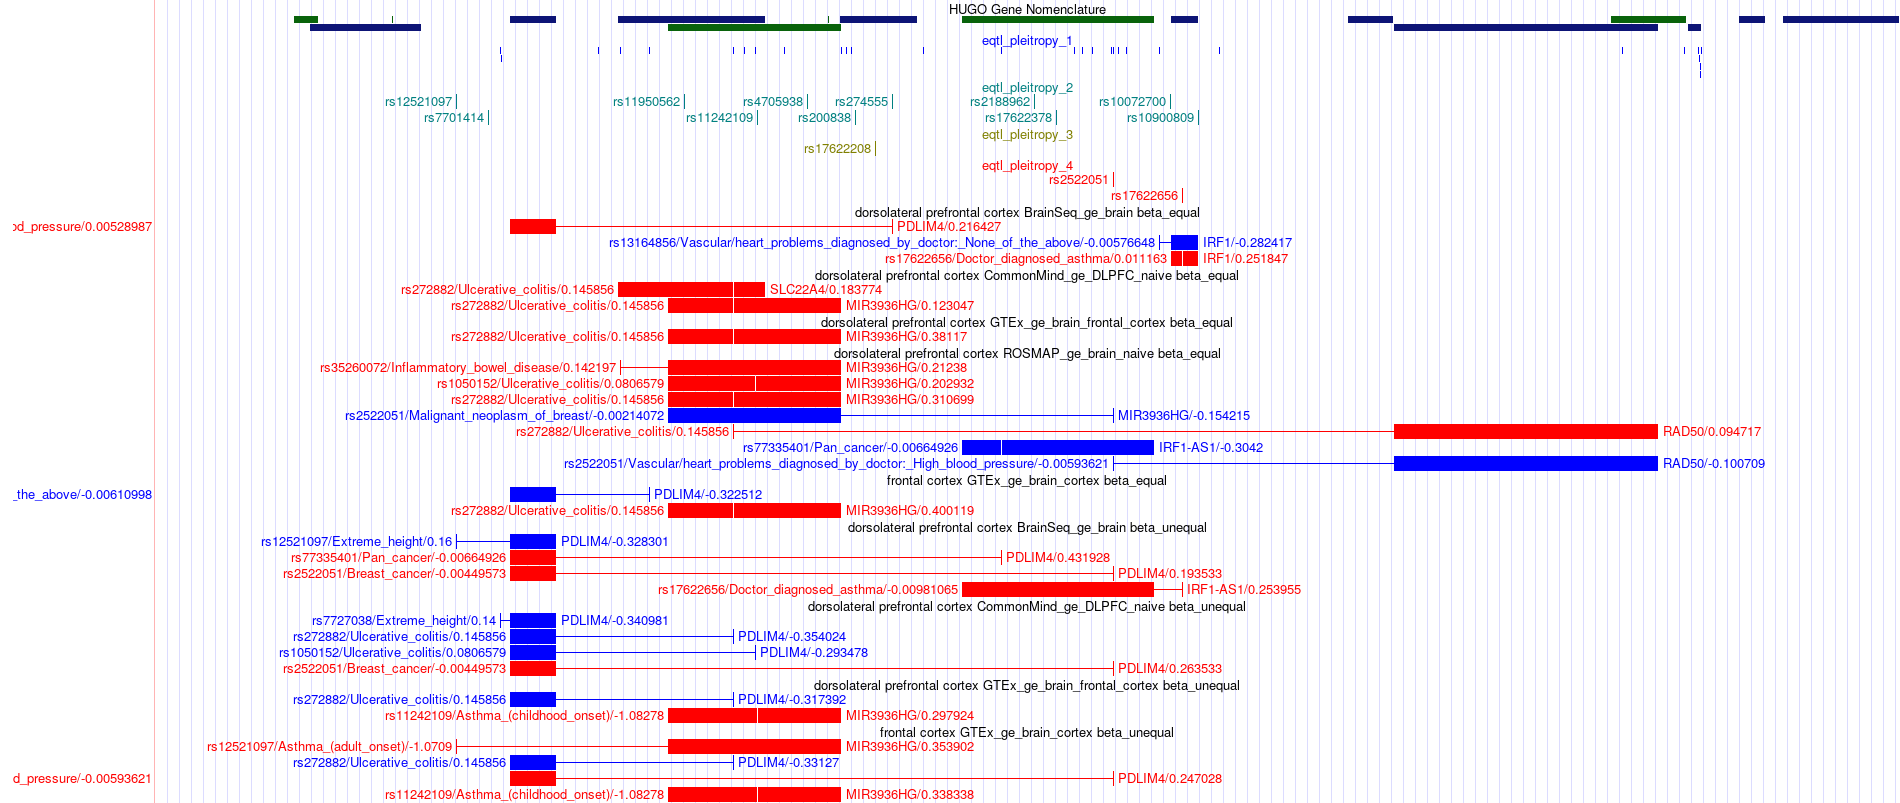
\includegraphics[width=\textwidth]{fig/ucsc_gwas2eqtl_il4_frontalcortex.png}
    \end{subfigure}

    \caption{}

\end{figure}

%%%%%%%%%%%%%%%%%%%%%%%%%%%%%%%%%%%%%%%%%%%%%%%%%%%%%%%%%%%%%%%%%%%%%%%%%%%%%%%%
%
% Fig 5: Comparison with Watanabe 2019
%
%%%%%%%%%%%%%%%%%%%%%%%%%%%%%%%%%%%%%%%%%%%%%%%%%%%%%%%%%%%%%%%%%%%%%%%%%%%%%%%%

\begin{figure}[!ht]
    %
    \centering
    %
    \begin{subfigure}[]{.49\textwidth}
        \textbf{a}
        \\
        \includegraphics[width=\textwidth]{\floatRelativePath/cmpt_count_per_rsid.py/watanabe_cat_count.png}
    \end{subfigure}
    %
    \begin{subfigure}[]{.49\textwidth}
        \textbf{b}
        \\
        \includegraphics[width=\textwidth]{\floatRelativePath/cmpt_count_per_rsid.py/watanabe_percentage.png}
    \end{subfigure}

    \caption{}

\end{figure}

%%%%%%%%%%%%%%%%%%%%%%%%%%%%%%%%%%%%%%%%%%%%%%%%%%%%%%%%%%%%%%%%%%%%%%%%%%%%%%%%
%
% Supp fig: allele frequencies
%
%%%%%%%%%%%%%%%%%%%%%%%%%%%%%%%%%%%%%%%%%%%%%%%%%%%%%%%%%%%%%%%%%%%%%%%%%%%%%%%%

\begin{figure}[!tbp]

    \begin{subfigure}[]{.32\textwidth}
        \textbf{a}
        \\
        \includegraphics[width=\textwidth]{\floatRelativePath/pltbar_x_per_gwas_cat_y_allele_freq.py/afr_af.png}
    \end{subfigure}
%
    \begin{subfigure}[]{.32\textwidth}
        \textbf{b}
        \\
        \includegraphics[width=\textwidth]{\floatRelativePath/pltbar_x_per_gwas_cat_y_allele_freq.py/amr_af.png}
    \end{subfigure}
%
    \begin{subfigure}[]{.32\textwidth}
        \textbf{c}
        \\
        \includegraphics[width=\textwidth]{\floatRelativePath/pltbar_x_per_gwas_cat_y_allele_freq.py/eas_af.png}
    \end{subfigure}

    \centering
    \begin{subfigure}[]{.32\textwidth}
        \textbf{d}
        \\
        \includegraphics[width=\textwidth]{\floatRelativePath/pltbar_x_per_gwas_cat_y_allele_freq.py/eur_af.png}
    \end{subfigure}
%
    \begin{subfigure}[]{.32\textwidth}
        \textbf{e}
        \\
        \includegraphics[width=\textwidth]{\floatRelativePath/pltbar_x_per_gwas_cat_y_allele_freq.py/sas_af.png}
    \end{subfigure}

    \caption{}

\end{figure}
